\label{ch:mg}

\section{Introduction to \maestro\ Multigrid}

\maestro\ uses multigrid to enforce the velocity constraint through
projections at the half-time (the MAC projection) and end of the time
step (the HG projection).  Two multigrid solvers are provided by
\boxlib---one for cell-centered data and one for node-centered (nodal)
data.  Both of these are used in \maestro.

\begin{figure}[t]
\centering
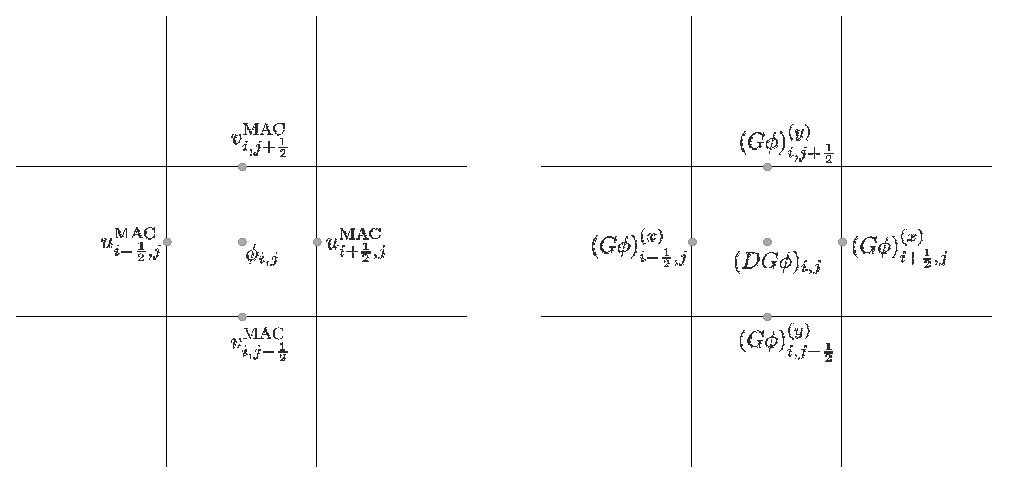
\includegraphics[width=5.5in]{\mgfigpath/MAC_mg2}
\caption{\label{fig:mg:MAC} Data centerings for the MAC projection}
\end{figure}

The MAC projection operates on the advective velocities predicted at
the cell-interfaces at the half-time.  The edge-centered velocities
are shown in Figure~\ref{fig:mg:MAC}.  If we consider purely
incompressible flow, the projection appears as:
\begin{equation}
D G \phi = D U
\end{equation}
where $D$ is the divergence operator and $G$ is the gradient operator.
In this discretization, $\phi$ is cell-centered (see
Figure~\ref{fig:mg:MAC}).  The remaining quantities are discretized as:
\begin{itemize}
\item $DU$ is cell-centered, 
  \begin{equation}
  (DU)_{i,j} = \frac{u_{i+1/2,j} - u_{i-1/2,j}}{\Delta x} + 
               \frac{v_{i,j+1/2} - v_{i,j-1/2}}{\Delta y}
  \end{equation}

\item $G\phi$ is edge-centered, on the MAC grid, as shown in
  Figure~\ref{fig:mg:MAC}.

\item $DG\phi$ is cell-centered, also shown in Figure~\ref{fig:mg:MAC},
  computed from $G\phi$ using the same differencing as $DU$.

\end{itemize}

\begin{figure}[t]
\centering
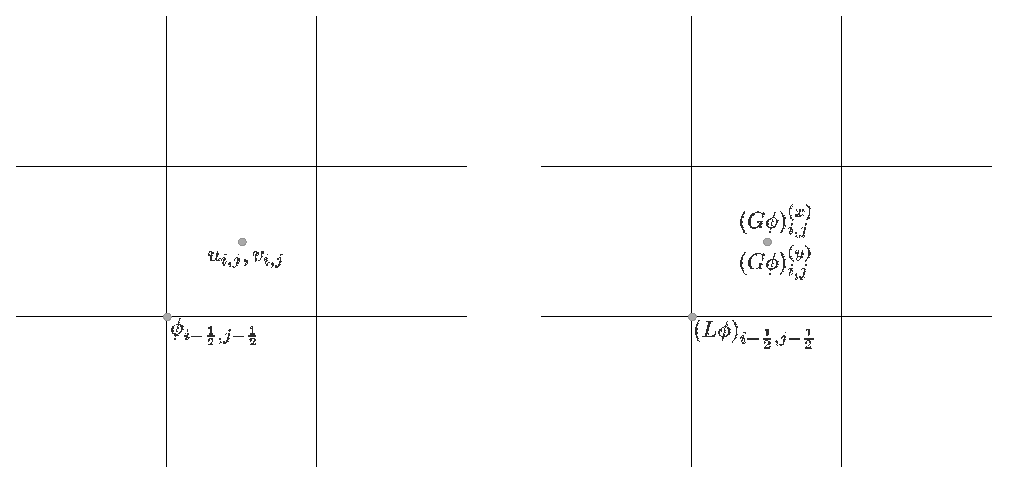
\includegraphics[width=5.5in]{\mgfigpath/HG_mg2}
\caption{\label{fig:mg:HG} Data centerings for the HG projection}
\end{figure}

The HG projection projects the cell-centered velocities at the end of
the timestep.  Here, $\phi$ is node-centered.  Figure~\ref{fig:mg:HG}
shows the locations of the various quantities involved in the HG
projection.  Again considering simple incompressible flow, we now
solve:
\begin{equation}
L \phi = D U
\end{equation}
where $L$ is a discretization of the Laplacian operator.  In this
sense, the HG projection is an {\em approximate projection}, that is,
$L \neq DG$ (in discretized form).  The various operations have the
following centerings:
\begin{itemize}

\item $DU$ is node-centered.  This is computed as:
  \begin{equation}
  (DU)_{i-1/2,j-1/2} = \frac{\frac{1}{2} (u_{i,j} + u_{i,j-1}) -
                             \frac{1}{2} (u_{i-1,j} + u_{i-1,j-1})}{\Delta x} +
                       \frac{\frac{1}{2} (v_{i,j} + v_{i-1,j}) -
                             \frac{1}{2} (v_{i,j-1} + v_{i-1,j-1})}{\Delta y} 
  \end{equation}

\item $G\phi$ is cell-centered, as shown in Figure~\ref{fig:mg:HG}.

\item $L\phi$ is node-centered.  This is a direct discretization of 
the Laplacian operator.  By default, \maestro\ uses a dense stencil
(9-points in 2-d, 27-points in 3-d).  Alternately, a {\em cross}
stencil can be used (by setting {\tt hg\_dense\_stencil = F}).  This
uses 5-points in 2-d, 7-points in 3-d.

\end{itemize}


\section{\mgtower}

The \mgtower\ is a special Fortran derived type that carries all the
information required for a \boxlib\ multigrid solve.

The following parameters are specified when building the \mgtower:
\begin{itemize}
\item {\tt smoother}: the type of smoother to use.  Choices are listed
  in {\tt mg\_tower.f90}.  Common options are {\tt
    MG\_SMOOTHER\_GS\_RB} for red-black Gauss-Seidel and {\tt
    MG\_SMOOTHER\_JACOBI} for Jacobi.

\item {\tt nu1}: The number of smoothings at each level on the way down
  the V-cycle.

\item {\tt nu2}: The number of smoothings at each level on the way up
  the V-cycle.

\item {\tt nub}: The number of smoothing before and after the bottom solver.

\item {\tt gamma}: \MarginPar{what does this mean?}

\item {\tt cycle\_type}: The type of multigrid to do, V-cycles ({\tt
  MG\_VCycle}), W-cycles ({\tt MG\_WCycle}), full multigrid ({\tt
  MG\_FCycle}).

\item {\tt omega}:  \MarginPar{description?}

\item {\tt bottom\_solver}: the type of bottom solver to use.  See the next
 section.

\item {\tt bottom\_max\_iter}: the maximum number of iterations for the 
  bottom solver

\item {\tt bottom\_solver\_eps}: the tolerance used by the bottom
  solver.  In \maestro, this is set via {\tt mg\_eps\_module}.

\item {\tt max\_iter}: the maximum number of multigrid cycles.

\item {\tt max\_bottom\_nlevel}: additional coarsening if you use
  {\tt bottom\_solver} type 4 (see below)

\item {\tt min\_width}: minimum size of grid at coarsest multigrid level

\item {\tt rel\_solver\_eps}: the relative tolerance of the solver (in
  \maestro, this is set via {\tt mg\_eps\_module}.

\item {\tt abs\_solver\_eps}: the absolute tolerance of the solver (in
  \maestro, this is set via {\tt mg\_eps\_module}.

\item {\tt verbose}: the verbosity of the multigrid solver.  In \maestro,
  this is set via the {\tt mg\_verbose} runtime parameter.  Higher
  numbers give more verbosity.

\item {\tt cg\_verbose}: the verbosity of the bottom solver.  In \maestro,
  this is set via the {\tt cg\_verbose} runtime parameter.  Higher
  numbers give more verbosity.

\end{itemize}

In addition to these parameters, the \mgtower\ carries a number of
\multifab s that carry the solution and stencil for the multigrid
solve.


\section{Bottom Solvers}

There are several bottom solvers available to \maestro.  These are set
through the {\tt mg\_bottom\_solver} (MAC) and {\tt
  hg\_bottom\_solver} (HG) runtime parameters.  The allowed values
  are:

\begin{itemize}

\item {\tt mg\_bottom\_solver} / {hg\_bottom\_solver} = 0: smoothing only.

\item {\tt mg\_bottom\_solver} / {hg\_bottom\_solver} = 1: biconjugate
  gradient stabilized---this is the default.

\item {\tt mg\_bottom\_solver} / {hg\_bottom\_solver} = 2: conjugate
  gradient method

\item {\tt mg\_bottom\_solver} / {hg\_bottom\_solver} = 4: a special 
  bottom solver that extends the range of the multigrid coarsening
  by aggregrating coarse grids on the original mesh together and
  further coarsening. \MarginPar{does this option then use bicg 
  at the new bottom?}

\end{itemize}

\MarginPar{any simple discussion on why we might choose one of the
  other bottom solvers?}

\subsection{Special Bottom Solver}
We have a special bottom solver type that greatly speeds up large problems
and speeds up smaller problems to a lesser degree.
In fact, you should use this bottom solver whenever possible, because I
have yet to find a case that performs worse than our standard bottom solver.
What this special solver essentially does is take the data from the coarsest 
level of the original multigrid V-cycle and copy it onto a new grid structure 
with the same number of total cells in each direction, but with a fewer number of larger 
grids.  A new V-cycle begins from this point, 
so we are essentially coarsening this ``new'' problem.
Now, the coarsest level of the multigrid V-cycle in the ``new'' problem has 
fewer cells and fewer grids as compared to the original coarsest level.

To enable this solver, set {\tt hg\_bottom\_solver = 4} (for the nodal
projections) and/or {\tt mg\_bottom\_solver = 4} (for the cell-centered
projections) in your inputs file.

To understand how this bottom solver works, the first thing you need to know
is what the grid structure of the coarsest level of your multigrid V-cycle
looks like (we need to put a description of this in the section above).
Now, figure out the size of the box you would need if you
wanted it to fit all the data on the coarsest level.  Now, figure out what
the largest integer $n$ is so that you can evenly divide the length of this box
by $2^n$ in every coordinate direction.  If $n < 2$, the program will abort
since the grid structure is not suitable for this bottom solver.

Now the code will set up a ``new'' problem, using the data at the coarsest level
of the original problem as the initial data.  The grid structure for this new
problem has the same number of cells as the coarsest level of the original problem,
but the data is copied onto a grid structure where each grid has $2^n$ cells
on each side.  The new V-cycle continues down to the new coarsest level, in
which each grid has 2 cells on each side.  If you wish to impose a limit on
the maximum value that $n$ can have, you can do so by setting 
{\tt max\_mg\_bottom\_nlevs} equal to that value.

{\bf Example 1:} A 3D problem with $384^3$ cells divided into $32^3$ grids, i.e., 
there is a $12\times 12\times 12$ block of $32^3$ grids.  The coarsest level of the 
multigrid V-cycle contains $12\times 12\times 12$ grids that have $2^3$ cells, so the 
entire problem domain has $24^3$ cells.  We see that $n=3$, and create a new problem 
domain with a $3\times 3\times 3$ block of $8^3$ grids.  The coarsest level of the 
multigrid V-cycle for the ``new'' problem will be a $3\times 3\times 3$ block of 
$2^3$ grids.

{\bf Example 2:} A 2D problem with $96\times 384$ cells divided into $48^2$ grids, i.e., 
there is a $2\times 8$ block of $48^2$ grids.  The coarsest level of the multigrid 
V-cycle contains $2\times 8$ grids that have $3^2$ cells, so the entire problem 
domain has $6\times 24$ cells.  We see that $n=1$, so the program aborts since this grid
structure is not appropriate for the fancy bottom solver.




\section{Convergence Criteria}

All \maestro\ multigrid solves consist of pure V-cycles.  


\section{Multigrid Solver Tolerances}

\label{sec:mgtol}

Beginning at the start of execution, there are several places where
either cell-centered multigrid or node-centered multigrid solves are
performed.  The outline below lists the solves one encounters, in order,
from the start of execution.  The values of the tolerances lists here
are defined in the {\tt mg\_eps} module.  To set problem-specific values
of these tolerances, place a local copy of {\tt mg\_eps.f90} in your
problem directory.

In the initialization, multigrid comes in during the initial projection
and the ``divu'' iterations.

\begin{itemize}

\item {\em initial projection} ({\tt initial\_proj} called from {\tt varden})

  The initial projection creates a first approximation to the velocity
  field by forcing the initial velocity field set by {\tt initveldata}
  to satisfy the elliptic constraint equation.  Since the initial
  velocity may be zero, there is no guarantee that a well-defined
  timestep can be computed at this point, so the source term, $S$,
  used here only involves thermal diffusion and any external heating
  term, $\Hext$---no reactions are included (see paper~III, \S 3.3).

  The initial projection can be disabled with the {\tt do\_initial\_projection}
  runtime parameter.

  The tolerances, {\tt eps\_init\_proj\_cart} and {\tt eps\_init\_proj\_sph}
  (for Cartesian and spherical respectively) are set in {\tt mg\_eps.f90}
  and have the default values of:
   \begin{center}
   \begin{tabular}{lll}
   Cartesian:   &  {\tt eps\_init\_proj\_cart} &= $10^{-12}$ \\
   spherical:   &  {\tt eps\_init\_proj\_sph}  &= $10^{-10}$
   \end{tabular}
   \end{center}


\item {\em ``divu'' iterations} ({\tt divu\_iter} called from {\tt varden})

  The ``divu'' iterations projects the velocity field from the initial
  projection to satisfy the full constraint (including reactions).
  This is an iterative process since the reactions depend on the
  timestep and the timestep depends on the velocity field (see
  paper~III, \S 3.3).  The number of iterations to take is set through
  the {\tt init\_divu\_iter} runtime parameter.

  The overall tolerance, $\epsilon_\mathrm{divu}$ depends on the iteration, $i$.
  We start with a loose tolerance and progressively get tighter.  The
  tolerances (set in {\tt divu\_iter}) are, for Cartesian:
  {\small
   \begin{center}
   \begin{tabular}{lll}
   $\epsilon_\mathrm{divu} = \left  \{ \begin{array}{lll} 
                   \min\, \{& \!\!\!\mathtt{eps\_divu\_cart} \cdot \mathtt{divu\_iter\_factor}^2 \cdot \mathtt{divu\_level\_factor}^{(\mathtt{nlevs}-1)}, \\
                            & \!\!\!\mathtt{eps\_divu\_cart} \cdot \mathtt{divu\_iter\_factor}^2 \cdot \mathtt{divu\_level\_factor}^2 \, \} & 
                           \quad \mathrm{for}~ i \le \mathtt{init\_divu\_iter} - 2 \\[2mm]
                   \min\, \{& \!\!\!\mathtt{eps\_divu\_cart} \cdot \mathtt{divu\_iter\_factor} \cdot \mathtt{divu\_level\_factor}^{(\mathtt{nlevs}-1)}, \\
                            & \!\!\!\mathtt{eps\_divu\_cart} \cdot \mathtt{divu\_iter\_factor} \cdot \mathtt{divu\_level\_factor}^2 \, \} & 
                           \quad \mathrm{for}~ i = \mathtt{init\_divu\_iter} - 1  \\[2mm]
                   \min\, \{& \!\!\!\mathtt{eps\_divu\_cart} \cdot \mathtt{divu\_level\_factor}^{(\mathtt{nlevs}-1)}, \\
                            & \!\!\!\mathtt{eps\_divu\_cart} \cdot \mathtt{divu\_level\_factor}^2 \, \} & 
                           \quad \mathrm{for}~ i = \mathtt{init\_divu\_iter}   \\
                                 \end{array}
                  \right .$ \\[10mm]
   \end{tabular}
   \end{center}
   }
   and for spherical:
   {\small 
   \begin{center}
   \begin{tabular}{ll}
   $\epsilon_\mathrm{divu} = \left  \{ \begin{array}{ll} 
                     \mathtt{eps\_divu\_sph} \cdot \mathtt{divu\_iter\_factor}^2 &
                           \quad \mathrm{for}~ i \le \mathtt{init\_divu\_iter} - 2 \, \\[2mm]
                    \mathtt{eps\_divu\_sph} \cdot \mathtt{divu\_iter\_factor}  & 
                           \quad \mathrm{for}~ i = \mathtt{init\_divu\_iter} - 1 \, \\[2mm]
                    \mathtt{eps\_divu\_sph}  &
                           \quad \mathrm{for}~ i = \mathtt{init\_divu\_iter} \, )\\
                  \end{array}
                  \right .$ \\
   \end{tabular}
   \end{center}
   }
   The various parameters are set in {\tt mg\_eps.f90} and have the default values of:
   \begin{center}
   \begin{tabular}{ll}
   {\tt eps\_divu\_cart}     &= $10^{-12}$ \\
   {\tt eps\_divu\_sph}      &= $10^{-10}$ \\
   {\tt divu\_iter\_factor}  &= 100 \\
   {\tt divu\_level\_factor} &= 10 
   \end{tabular}
   \end{center}

\end{itemize}

In the main algorithm, mulitgrid solves come in during the two MAC projections,
two (optional) thermal diffusion solves, and the final velocity projection.

\begin{itemize}

\item {\em MAC projection}  

  The MAC projection forces the edge-centered, half-time advective
  velocities to obey the elliptic constraint.  This is done both in
  the predictor and corrector portions of the main algorithm.

  There are two tolerances here.  The norm of the residual is required
  to be reduced by a relative tolerance of $\epsilon =
  \min \{ \mathtt{eps\_mac\_max}, \mathtt{eps\_mac} \cdot
  \mathtt{mac\_level\_factor}^{(\mathtt{nlevs}-1)} \}$. A separate
  tolerance is used for the bottom
  solver, $\epsilon_\mathrm{bottom} =
  \mathtt{eps\_mac\_bottom}$.  These parameters are set in {\tt
    mg\_eps.f90} and have the default values:
   \begin{center}
   \begin{tabular}{ll}
   {\tt eps\_mac}           &= $10^{-10}$ \\
   {\tt eps\_mac\_max}           &= $10^{-8}$ \\
   {\tt mac\_level\_factor} &= 10 \\
   {\tt eps\_mac\_bottom}   &= $10^{-3}$
   \end{tabular}
   \end{center}


  %an absolute tolerance of $\epsilon_\mathrm{abs} =
  %\epsilon \cdot ||U^\mathrm{ADV}||_\infty / \Delta x$

\item {\em thermal diffusion}

  This uses the same {\tt mac\_multigrid} routine as the MAC
  projection, so it uses the same tolerances.  The only difference is
  that the absolute tolerance is based on the norm of $h$ now, instead
  of $U^\mathrm{ADV}$.

\item {\em velocity projection}

  The final velocity projection uses a tolerance of $\epsilon = \min \{
  \mathtt{eps\_hg\_max}, \mathtt{eps\_hg} \cdot \mathtt{hg\_level\_factor}^{(\mathtt{nlevs} - 1)} \}$.  This tolerance
  is set in {\tt hgproject} using the parameter values specified in {\tt mg\_eps.f90}.  A separate
  tolerance is used for the bottom
  solver, $\epsilon_\mathrm{bottom} = \mathtt{eps\_hg\_bottom}$.


  The default parameter values are:
   \begin{center}
   \begin{tabular}{ll}
   {\tt eps\_hg}     &= $10^{-12}$ \\
   {\tt eps\_hg\_max}      &= $10^{-10}$ \\
   {\tt hg\_level\_factor}  &= 10 \\
   {\tt eps\_hg\_bottom}   &= $10^{-4}$
   \end{tabular}
   \end{center}

\end{itemize}


\section{General Remarks}

If \maestro\ has trouble converging in the multigrid solves, try
setting the verbosity {\tt mg\_verbose} or {\tt cg\_verbose} to
higher values to get more information about the solve.
